\subsection{Results and discussion}\label{sec:m2:results} 

    \subsubsection{Times and sound horizon}
    The relevant times for last scattering, recombination and Saha recombination are obtained as explained in ~\cref{sec:m2:methods:analysis}, and presented in ~\cref{tab:m2:recomb_analysis}. These times are given in terms of $x$, the redshift $z$ and the cosmic time $t$ (in Myr). The sound horizon is given in units of megaparsecs (Mpc). Last scattering occurred when $x=-6.9853$, at redshift $z=1079.67$, which is slightly after recombination when $x=-6.9855$ at redshift $z=1079.83$. If the Saha approximation was valid when the electron fraction dropped, recombination would have happened when $x=-7.1404$ at redshift $1260.89$ which is significantly earlier. However, this is not the case since photons drop out of equilibrium with the primordial plasma as soon as hydrogen begin to form, and the free electron fraction is reduced. Thus, this number may only be used for comparison. Another thing worth noting is the validity of these numbers.
    \begin{table}
        \label{tab:m2:recomb_analysis}
        \begin{tabular}{l|rrrr}
\hline
Phenomenon & $x$ & $z$ & $t$ [Myr] & $r_s$ [Gyr] \\
\hline
Last scattering   & -6.99 & 1082.29 & 0.377 & 55394.8 \\
Recombination     & -6.99 & 1079.83 & 0.378 & 55590.6 \\
Saha              & -7.14 & 1260.89 & 0.291 & 43620.6 \\
\hline
\hline
\end{tabular}

        \caption{The times of last scattering and recombination given in terms of $x$, the redshift $z$, the cosmic time $t$ and the sound horizon $r_s$. Also included is the time of recombination found using the Saha approximation only.}
    \end{table}

    \subsubsection{Free electron fraction}
    ~\cref{fig:m2:electron_fraction} shows the free electron fraction $X_e$ as a function of $x$ found using both the Saha and Peebles equation, as explained in ~\cref{sec:m2:methods:electron_fraction}, in blue. Also shown is the results found from the Saha equation only, which tends to zero a lot faster. This is used for comparison only, as we have already stated that the Saha approximation is only valid for $X_e\simeq 1$. The time of recombination is shown for both cases, which for the Saha approximation happens significantly earlier than what is the actual case. The Peebles solution falls off gradually, and converges towards a constant value, which is the present day abundance of free electrons (freeze out abundance). This is found to be $X_e(x=0) = 0.0002$, shown as a brown dashed line in ~\cref{fig:m2:electron_fraction}.

    Since the Peebles equation is a solution of the Boltzmann equation, it takes into account the particle interaction with changing abundance, after the photons decouple from the primordial plasma. It is thus expected that this will result in a much more gradual fall off of the free electron fraction, just as we observe in ~\cref{fig:m2:electron_fraction}.
    \begin{figure}
        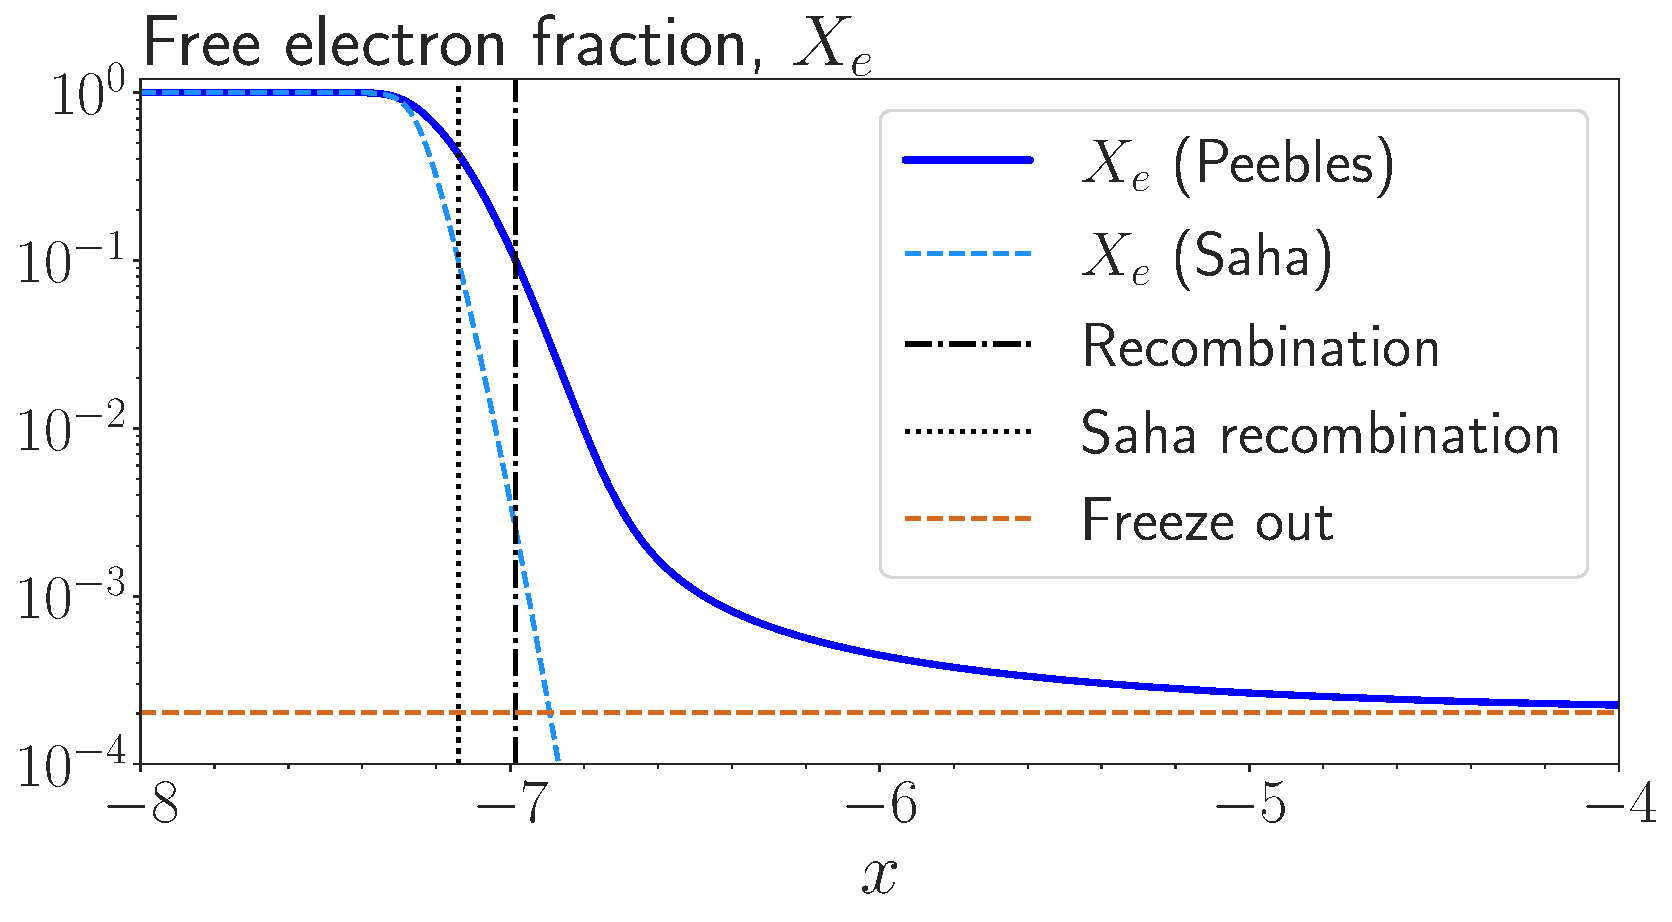
\includegraphics[width=\linewidth]{Xe_plot.pdf}
        \caption{The free electron fraction $X_e$ as function of $x$, found from the Saha and Peebles equation (blue). The result using only the Saha equation is shown in dashed light blue. The time of recombination is shown as a dashed black line. Likewise, recombination in the Saha approximation is shown as a dotted black line, appearing earlier. The freeze out abundance of hydrogen (the present value) is shown as a brown dashed line.}
        \label{fig:m2:electron_fraction}
    \end{figure}

    \subsubsection{Visibility}

    ~\cref{fig:m2:optical_depth} shows the optical depth and its first two derivatives as functions of $x$. This is a function of the time $x$, and thus the optical depth at some value is the integral of ~\cref{eq:m2:theory:optical_depth} from that time until today; it is cumulative. The surface of last scattering is shown with a black dashed line, before which the primordial plasma is optically thick, meaning the photons have a short mean free path. The decrease of the optical depth means that the photons gradually travel longer distances before interacting with free electrons. There are two processes going on here; the expansion of space itself, and the formation of neutral hydrogen. Both of which contribute to the increased mean free path of the photons. The contribution from the expansion of space is slow compared to the seemingly rapid change in the free electron fraction once neutral hydrogen is able to form. Thus, the rapid decrease of free electrons, as seen is ~\cref{fig:m2:electron_fraction} makes the mean free paths of photon to increase beyond the horizon. This effectively enable them to travel through space without interacting with matter, and this is what we observe as the CMB today - the Universe becomes transparent. This sudden decrease of optical depth is clearly seen in ~\cref{fig:m2:optical_depth}, both in $\tau$ itself, but also in its derivatives.
    \begin{figure}
        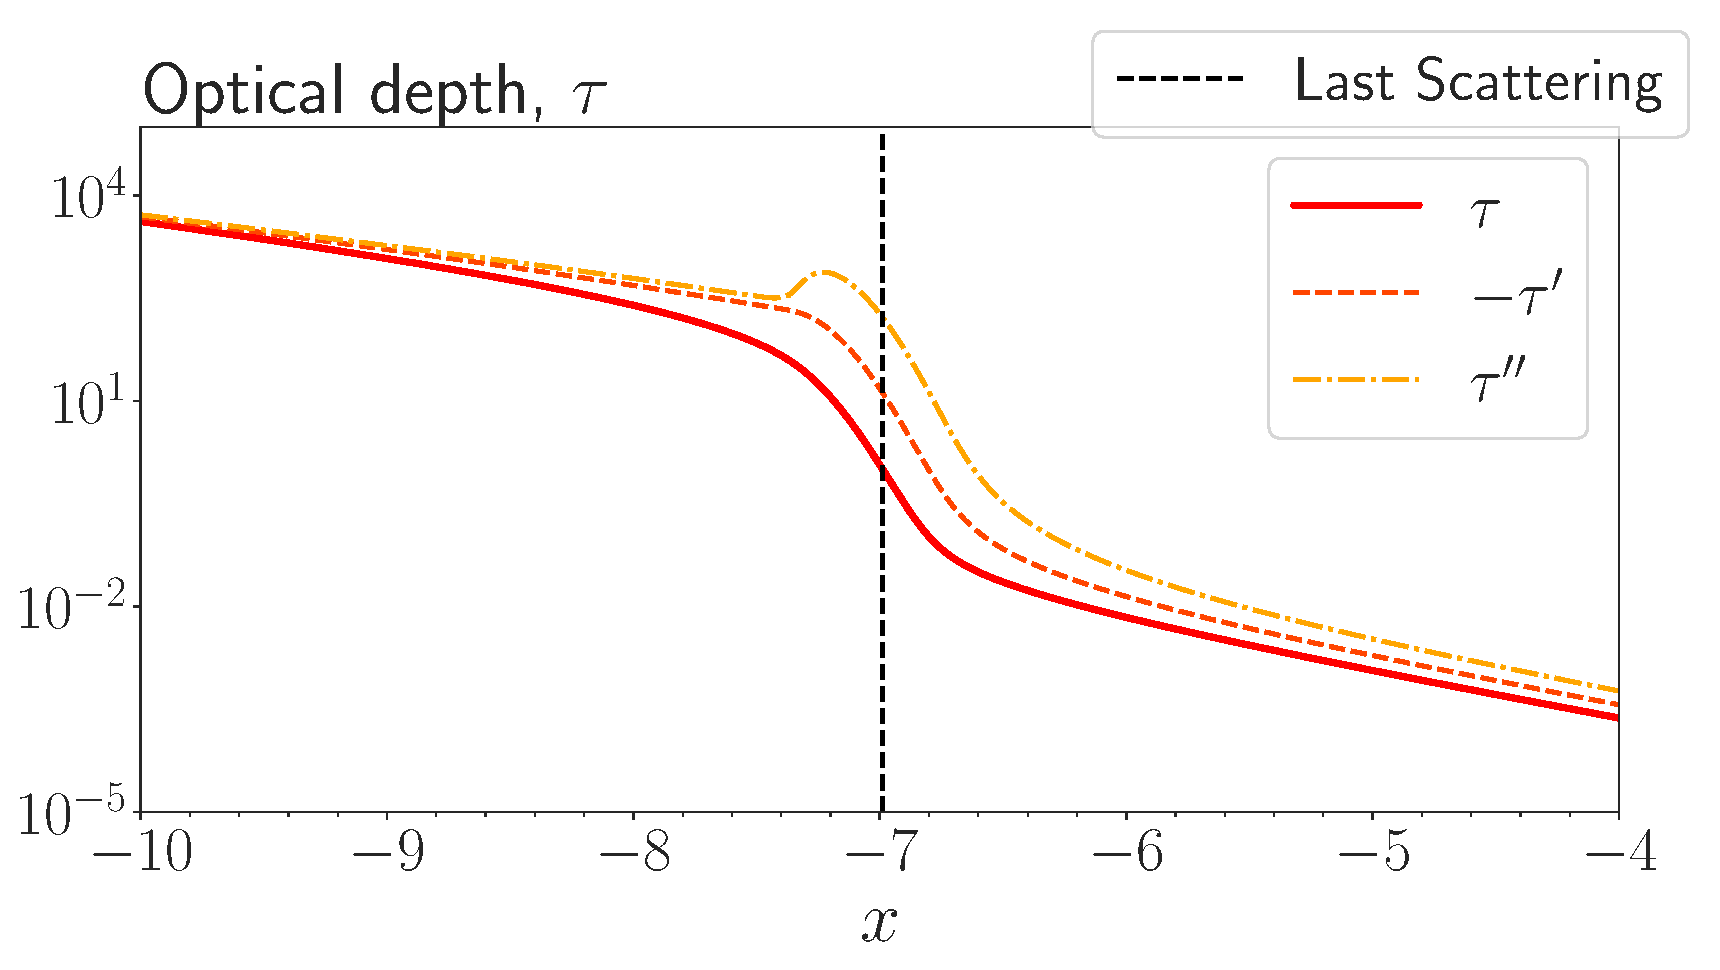
\includegraphics[width=\linewidth]{optical_depth.pdf}
        \caption{The optical depth $\tau$ and its first and second derivatives as functions of $x$. The time of last scattering is shown as a dashed black line, before which the Universe was optically thick.}
        \label{fig:m2:optical_depth}
    \end{figure}

    Another way of arriving at similar conclusions is by considering the visibility function in ~\cref{fig:m2:visibility_function}. Here, $\tilde{g}$ is shown in green along with its derivatives. The scaling follow that of ~\cite{https://doi.org/10.48550/arxiv.astro-ph/0606683}, in order to fit the graphs into the same figure. $\tilde{g}$ describes the probability that a photon reaching us today scattered at time $x$. The peak of this function indicates the time were \textit{the most} photons scattered for the last time, and is thus used as a definition of the last scattering surface. The visibility function is skewed forward in time.
    \begin{figure}
        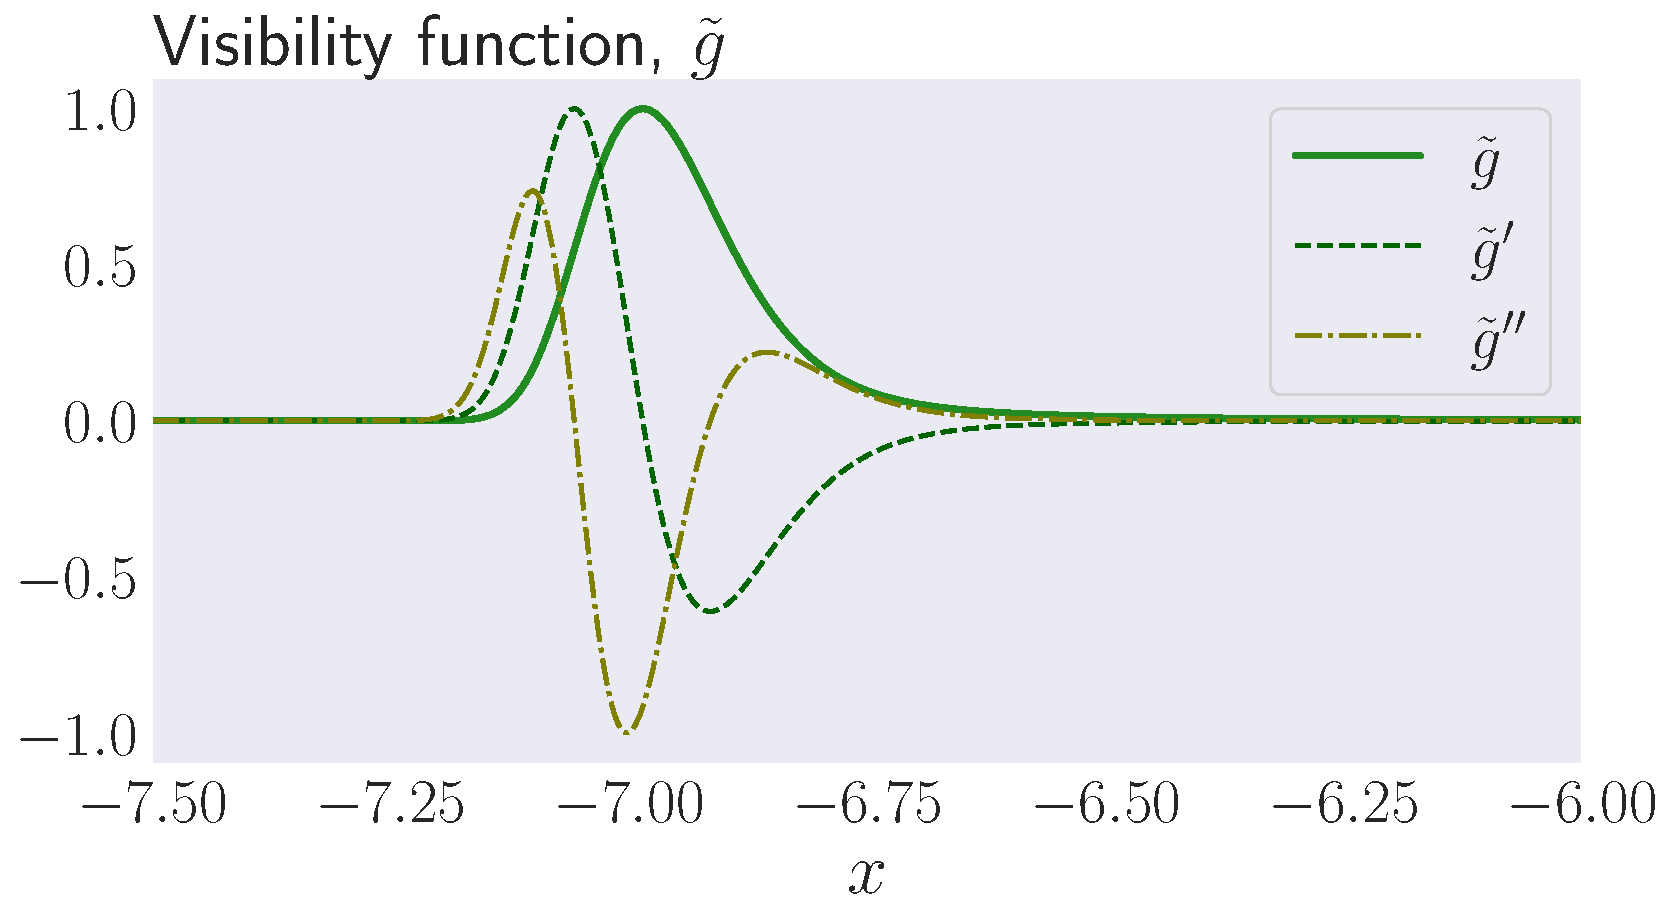
\includegraphics[width=\linewidth]{visibility_function.pdf}
        \caption{The visibility function $\tilde{g}$ and its first and second derivatives as functions of $x$. The time of last scattering is shown as a dashed black line, which by definition coincides with the peak of the visibility function.}
        \label{fig:m2:visibility_function}
    \end{figure}

    \subsubsection{General discussion}
    One key thing to keep in mind is that recombination did not happen instantaneously, but rather over a relatively short period in which neutral hydrogen formed rapidly. This caused a rapid decrease of the free electron fraction, which again caused the optical depth to decrease by several magnitudes. In the same period, we see a that the visibility function is non-zero, meaning the probability of last scattering is (relatively) very high in this period. The times quoted in ~\cref{tab:m2:recomb_analysis} are times that arise from our quite rigid, but fair definition of last scattering and recombination. However, these times do not encapsulate the duration of the abovementioned period.  One could also define the last scattering surface as the time when $\tau=1$ which is the transition between optically thick and optically thin media (when the photon travels exactly one mean free path before scattering). However, the visibility function is arguably a better choice since this is a proper probability distribution, so its peak represents the \textit{actual} time when the probability of last scattering was the highest. Nevertheless, if we change these definitions we ought to expect different times as a result.

